% 旋转构造 例2：等边△ABC 内一点 P, PA=5, PB=4, PC=3, 求 ∠BPC=150°
\documentclass[tikz,border=4pt]{standalone}
\usepackage{ctex}
\usepackage{amsmath}
\usetikzlibrary{calc, decorations.markings}
\begin{document}
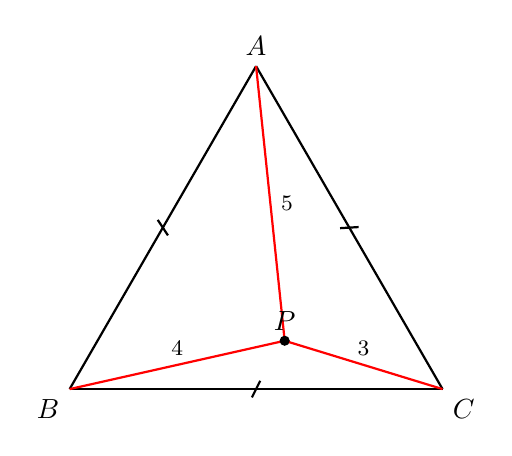
\begin{tikzpicture}[scale=0.7, thick,
  tick/.style={postaction={decorate, decoration={markings,
    mark=at position 0.5 with {\draw (-1.5pt,-3pt) -- (1.5pt,3pt);}}}}]
  % 等边边长 a. 由 PA=5, PB=4, PC=3 -> a²?
  % 已知费马点/旋转结论: 旋转后 △BPP' 等边 PP'=4, △CPP' 边 3,4,5 直角
  % a可由余弦定理算: 设 P 坐标. 不需精确, 示意即可
  % 估 a ≈ 6.766 (由公式 a² = (PA²+PB²+PC²+4√3 S)/2 等)
  % 简单做：a=6.766, B=(0,0), C=(a,0), A=(a/2, a*√3/2). 直接计算 P:
  % PA²=25, PB²=16, PC²=9
  % 设 P=(x,y). x²+y²=16 (PB), (x-a)²+y²=9 (PC), (x-a/2)²+(y-a√3/2)²=25
  % 前两式: -2ax+a²=-7 -> x=(a²+7)/(2a)
  % 第3-第1: -ax-a√3 y + a² = 9 -> ax + a√3 y = a²-9
  % => x + √3 y = a - 9/a
  % 用 x²+y²=16. 也可直接给出 a 数值:
  % 实际 a² 通过求和: 2a^2 = PA²+PB²+PC²+ ... 不重要 - 示意图
  \def\a{6.766}
  \coordinate (B) at (0,0);
  \coordinate (C) at (\a,0);
  \coordinate (A) at ({\a/2}, {\a*0.866});
  % 计算 P
  % x = (a²+7)/(2a) = (45.8+7)/13.53 = 3.902
  % from x²+y²=16 => y² = 16 - 15.23 = 0.77 -> y=0.877  (但应在三角形内, 检验)
  \coordinate (P) at (3.902, 0.877);
  \draw[tick] (A)--(B);
  \draw[tick] (B)--(C);
  \draw[tick] (C)--(A);
  \draw[red] (A)--(P);
  \draw[red] (B)--(P);
  \draw[red] (C)--(P);
  \filldraw (P) circle (2pt);
  \node[above] at (A) {$A$};
  \node[below left] at (B) {$B$};
  \node[below right] at (C) {$C$};
  \node[above] at (P) {$P$};
  \node at ($(A)!0.5!(P) + (0.3, 0)$) {\footnotesize $5$};
  \node at ($(B)!0.5!(P) + (0, 0.3)$) {\footnotesize $4$};
  \node at ($(C)!0.5!(P) + (0, 0.3)$) {\footnotesize $3$};
\end{tikzpicture}
\end{document}
